\section[Feature Spaces in Machine Learning]{Sidebar: Feature Spaces in Machine Learning}\label{sb:featspace}
Suppose we have data $\sampSetClass = \sampSetClassLong$, where $x_i\in\domI$ and $y_i\in\domO$. Here, $\domI$ is the input domain, and 
is generally a subset of $\R^D$, although more general sets such as discrete spaces, graphs, or text documents can be considered.
Similarly, $\domO$, the output domain, can be just as general as $\domI$. We wish to solve for functions $f$ in some space 
of functions $\functionSet$ such that $f(x_i) = y_i \ \forall i$. Generally, to restrict the complexity of the space $\functionSet$,
a \emph{loss function} $L(f, \sampSetClass)\mapsto\R$ is chosen, which measures the error between a prediction $f(x_i)$ given a datapoint 
$x_i$, and $y_i$, averaged over the entire dataset $\sampSetClass$, and the optimization problem becomes 
\begin{align}
 f^* = \argmin_{\functionSet}L(f, \sampSetClass) + \la g(f),
\end{align}
where $\la\in\R$, and $g(f)$ represent some constraints on the function $f$, such as smoothness. 
Control theorists are most likely familiar with 
input-output pairs where $x_i\in\R^N$ and $y_i$ is either in $\R$ or $\R^M$ (\emph{regression}). 
In machine learning, the most common task is when the $y_i$ are discrete (\emph{classification}). 
Different combinations of task, loss functions, and spaces $\functionSet$ result in different algorithms to solve these problems,
which can sometimes form entire subfields of machine learning. 

The choice of the function space $\functionSet$ can be critical for the task we want to perform,
similar to how the choice of the state space is in control theory. Let's consider a simple
example. Suppose we have data from two \emph{classes} $\sampSetClass_A = \{(x_1^A, y_1^A), \dots, (x_N^A, y_N^A)\}$ and 
$\sampSetClass_B = \{(x_1^B, y_1^B), \dots, (x_N^B, y_N^B)\}$, where $x_i^{\{A,B\}}\in\R^D$, and $y_i^{\{A,B\}}\in\{-1,+1\}$, shown
in Figure \ref{fig:lisep_data}. Let $f$ be chosen from the class of linear algorithms, i.e. $f = w^Tx + b$, where $w\in\R^D, b\in\R$. 
We pick a loss $L$ that returns a loss of zero when the prediction is the correct class, and if the prediction is the incorrect class,
returns a higher value for misclassifications that are closer to the boundary. A classical example of such a loss is that used by
the \emph{perceptron algorithm}, which can be written as 
\begin{align}\eqlabel{perc_loss}
 L(f, \sampSetClass) = \frac{1}{\nsamp}\sum_{i=1}^N\max(0, -y_iw^Tx). 
\end{align}
This loss measures how accurate the prediction of the perceptron is on average. The general algorithm is as follows:
\begin{enumerate}
 \item Initialize $\weight\in\R^D$ to all zeros. 
 \item For a fixed number of iterations, or until some stopping criterion is met:
       \begin{enumerate}
        \item For each training example $(x_i, y_i)$,
              \begin{enumerate}
               \item Let $\hat{y}_i=\sgn(\weight^Tx_i)$.
               \item If $y_i\neq\hat{y}_i$, update $\weight \leftarrow \weight + y_ix_i$.
              \end{enumerate}
       \end{enumerate}
\end{enumerate}
%This outline of the algorithm will be referenced later when we examine the nonlinear version of it.
The perceptron was one of the first machine learning models, and the genesis of modern neural networks \cite{rosenblatt1958perceptron}. 
Figure \ref{fig:linsep} shows a visual representation of where the perceptron algorithm can solve for the decision boundary with zero error. 
However, if the structure of the data has some nonlinearities, no solution will be found, as seen in Figure \ref{fig:nlinsep}. In this case,
the original space the data resides in is, in some sense, not a rich enough representation. If we could construct a mapping of the data to a
different space which gives a learning algorithm more degrees of freedom to work with, linear algorithms can still be deployed. 
If we map the same data using a nonlinear map $\phi(x,y):= (x^2, y^2, 2xy)$, the perceptron now finds a solution
in 3 dimensions, as seen in Figure \ref{fig:fmapped}. This example shows why so much of the work in machine learning focuses on 
learning the right representation for the data, for the right representation makes the classification task easy. Two major threads of 
research in the arena of feature maps over the last 40 years are kernel methods, and neural networks, the latter
of which has gained remarkable notoriety in the last 10 years. 
%Decision tree learning methods such as gradient boosting and random forests
%arose from the statistics community and enjoy significant adoption in industry \cite{Wasserman}, but will not be described in this work.  
These lines of research represent distinctly different strategies for generating feature maps from data. 

In Figure \ref{fig:nlinsep}, the data was mapped using an explicit feature map. Kernel methods utilize an elegant strategy for generating
feature maps from data, using a remarkably simple trick called \emph{the kernel trick}. Given a positive-definite kernel function 
$\kernel(x,y):\dom\times\dom\to\R$, Mercer's theorem guarantees the existence of a feature map $\fmap:\dom\to\fspace$, where $\fspace$
is a \emph{reproducing kernel Hilbert space (RKHS)}, and the map $\fmap$ obeys the property 
\begin{align}\eqlabel{kmap}
 \kernel(x,y) = \l\fmap(x), \fmap(y)\r_{\fspace}.
\end{align}
Recall that since $\fspace$ is an RKHS, given $c\in\dom$, $\kernel(x, c) = \l\fmap(x), \fmap(c)\r_{\fspace}$, 
and $\kernel(x, c) := \fmap_c\in\fspace$. Furthermore, $\Span\{\fmap_x\}_{x\in\dom}$ is dense in $\fspace$. There exist kernels 
that generate $\fspace$s that are extremely high dimensional: for example, the RBF kernel $\kernel(x,y) = e^{-\gamma\|x-y\|^2}$
is infinite-dimensional. This high degree of freedom enables the design of powerful learning algorithms that are linear in $\fspace$,
but nonlinear in the input domain $\dom$. The canonical example of this is the support vector machine (SVM) \cite{cortes1995support},
but a more instructive example for us is the perceptron algorithm. 


Suppose we trained a percetron using $\sampSet=\sampSetLong$, $x_i\in\R^D$ for some $D$, $y_i\in\{-1, 1\}$.
The prediction of the perceptron is $\hat{y}=\sgn(w^Tx)$, where $\weight\in\R^D$. It can be shown that 
$\weight=\sum_{i=1}\alpha_iy_ix_i$, where $\alpha_i$ is the number of times $x_i$ was misclassified. This allows us
to derive the dual version of this algorithm, because
\begin{align*}
 \hat{y} = \sgn(\weight^Tx) = \sgn\sum_{i=1}^n\al_iy_i\l x_i, x\r_{\R^D}.
\end{align*}
The dot product $\l x_i, x\r_{\R^D}$ can be replaced with the kernel, leading to the \emph{kernel perceptron algorithm}:
\begin{enumerate}
 \item Initialize $\alpha\in\R^{\nsamp}$ to all zeros. 
 \item For a fixed number of iterations, or until some stopping criterion is met:
       \begin{enumerate}
        \item For each training example $(x_j, y_j)$,
              \begin{enumerate}
               \item Let $\hat{y}_i=\sgn\sum_{i=1}^n\al_iy_i\kernel(x_i, x_j)$.
               \item If $y_i\neq\hat{y}_i$, update $\alpha_j \leftarrow \alpha_j + 1$.
              \end{enumerate}
       \end{enumerate}
\end{enumerate}
%Note that the computation time associated with these types of algorithms grows with the number of data points $\nsamp$, which
%means they are, in dual form, nonparametric. 
This algorithm is nonlinear in the input domain, but linear in the feature space $\fspace$, which led the deep learning community to,
somewhat pejoratively, label this as an example of a \emph{shallow learning architecture}.
Kernel methods can also be used in a more direct fashion: if we have a subspace $\fspace'\subset\fspace$ with a basis generated
from $\shCent = \shCentLong$, i.e. $\fspace' = \Span\{\fmap_{c_1},\dots,\fmap(c_{\ncent})\}$,
a linear model in $\fspace'$ is again given
by a vector $\weight\in\R^{\ncent}$. Suppose this weight vector represents a boundary in $\fspace'$: 
to compute which side of this boundary a point $x$ would lie on in $\fspace'$,
we simply compute $\sgn(\sum_{i=1}^{\ncent}\weight_i\l\fmap(x), \fmap(c_i) \r_{\fspace}) = \sgn(\sum_{i=1}^{\ncent}\weight_i\kernel(x,c_i))$.
The choice of the kernel and its parameters
depends on the dataset and the loss function. The kernel and the data together form the feature space. Because kernel methods are linear
in their parameters and are restricted to RKHSs, they are amenable to somewhat straightforward mathematical analysis, and are very well
studied because of this. 

Deep neural networks (DNNs) are algorithms where the function $f$ has nested nonlinearities. Fix a width $\ncent\in\mathbb{N}$. Deep nets are
parameterized models with 
weight matrices $W^l\in\R^{\ncent\times\ncent}$, bias vectors $b^l\in\R^{\ncent}$, and a pointwise nonlinearity $\phi:\R\to\R$, 
with $l=1,\dots,L$. Vectors $h^l\in\R^{\ncent}$ are called preactivations, and $x^l\in\R^{\ncent}$ are called postactivations,
each element of which is called a \emph{neuron}. 
Let $h^0\in\R^{\ncent}$ be the input: then the canonical feedforward neural network is given by 
\begin{align}
 x^l = \phi(h^l), \ h^l = W^lx^{l-1} + b^l.
\end{align}
Therefore, we have that $f(h^0) = x^l$. The individual steps $l$ are called the \emph{layers} of the network, and the nesting property
allows these networks to learn much more complicated functions than shallow architectures given the same number of nonlinearities 
\cite{bengio2009learning}. Different choices of nonlinearities, connections, and layer architectures lead to different types of
neural networks, which are used for different applications \cite{goodfellow2016deep}. Deep learning has had an enormous impact on
both the machine learning literature and industrial applications, and that impact has bled over rapidly to other fields. Due to
the nested structure of nonlinearities in DNNs, they are more difficult to analyze using simple mathematical tools, and therefore
most of the literature in the field has focused on the empirical performance of these methods, where they significantly outperform 
competing methods. 

The signal acheivement of machine learning in general and deep learning in particular has been its ability to weaponize computation
to obliterate the obstacles nexessary for industrial progress. Control needs to provide insight into the structure of the spaces
these models generate, to restrict certain forms of output, and to shape decision-making. 

\begin{figure}\label{fig:linsep}
\centering
    \subfloat[Data from classes $A$ and $B$.]
    {
    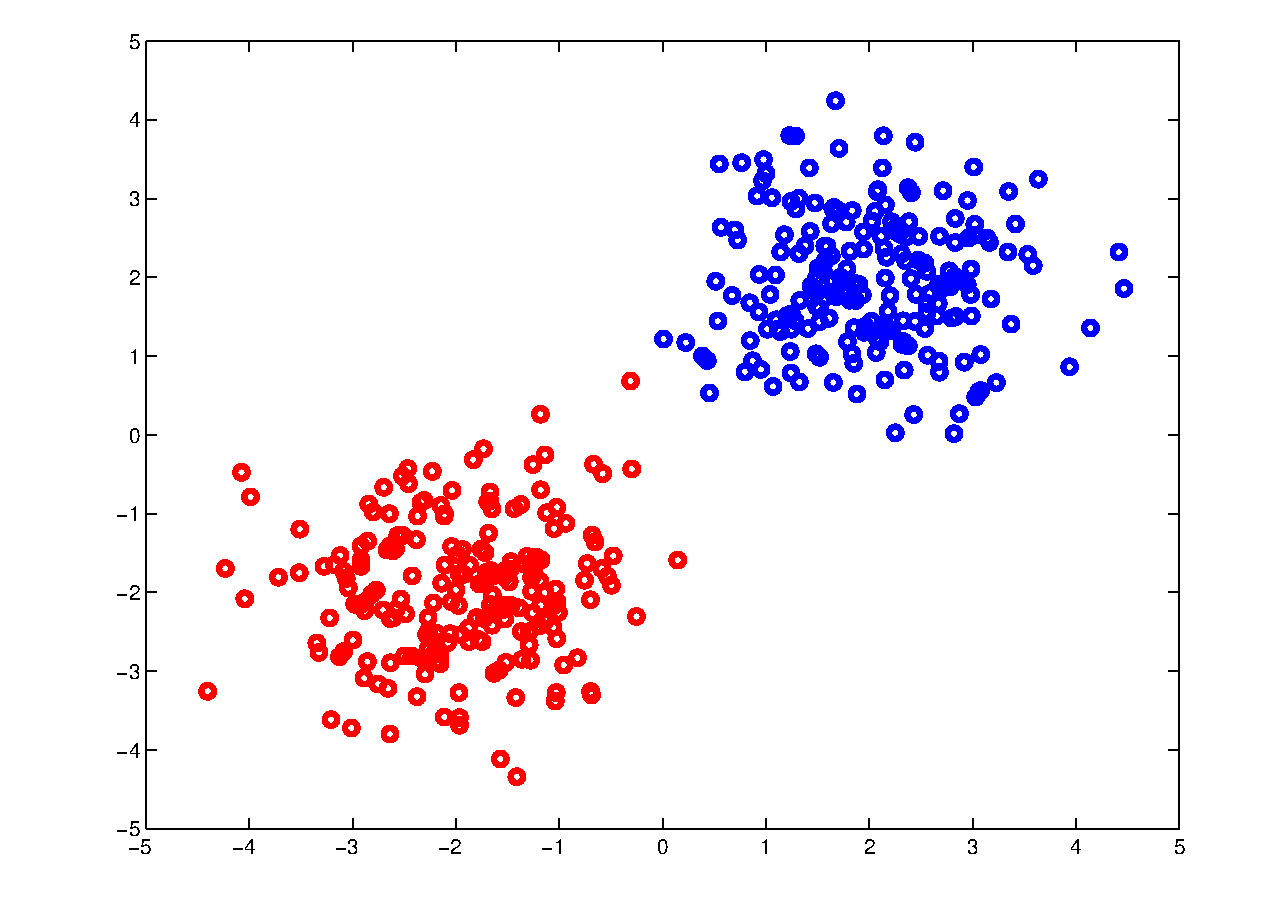
\includegraphics[width=0.45\columnwidth]{figures/linsep_data.pdf}
    \label{fig:lisep_data}}
     \subfloat[Linear boundary separating data.]
     {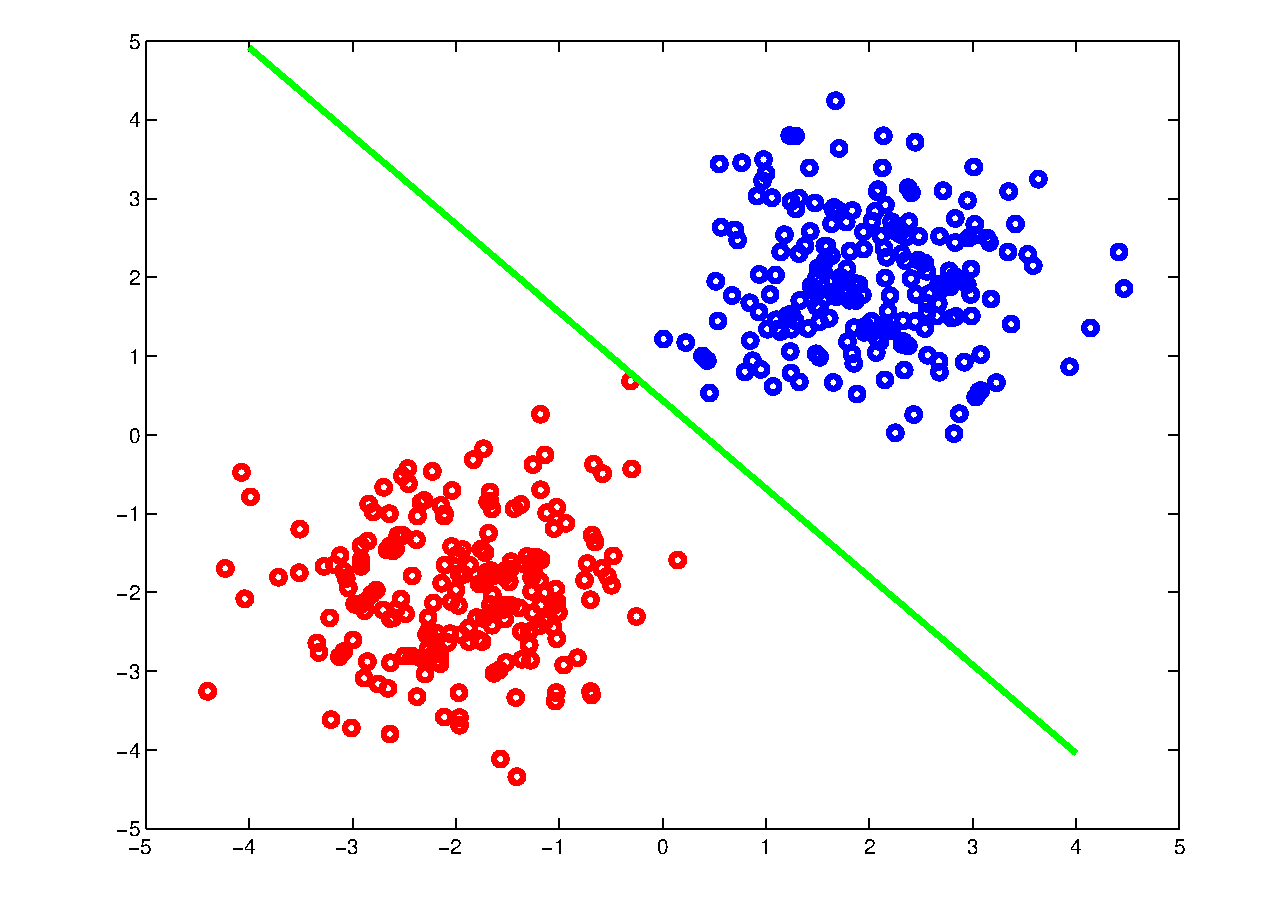
\includegraphics[width=0.45\columnwidth]{figures/linsep_data_perceptron.pdf}
     \label{fig:lin_sep_bound}}  
    \caption{Example of linearly separable data. Any simple linear learning algorithm e.g. perceptron, finds a solution.}
    \label{fig:linsep}
    %\end{figure}
%\begin{figure}[tbh] %{r}{0.5\textwidth}
\end{figure} 

\begin{figure}
\centering
    \subfloat[Data from classes $A$ and $B$.]
    {
    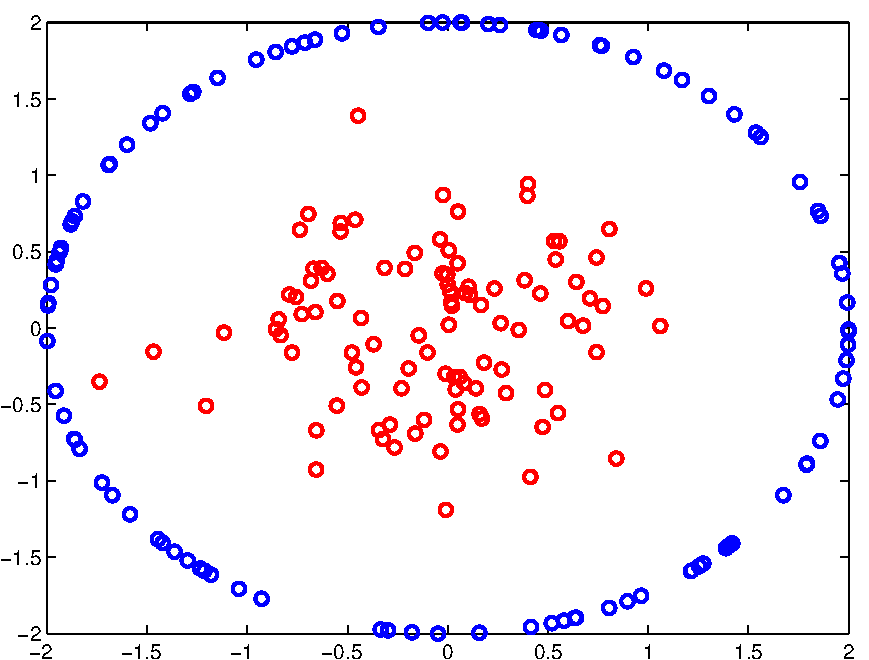
\includegraphics[width=0.45\columnwidth]{figures/pres_original_data.pdf}
    \label{fig:nlisep_data}}
     \subfloat[Linear boundary fails to separate data.]
     {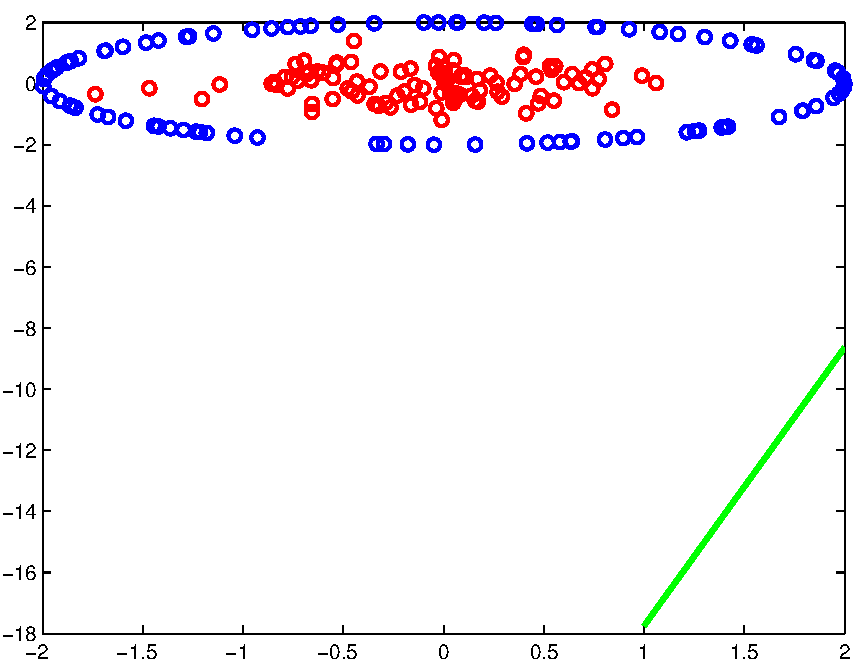
\includegraphics[width=0.45\columnwidth]{figures/pres_perc_original_data.pdf}
     \label{fig:nlin_sep_bound}}  
    \caption{Example of nonlinearly separable data. Perceptron fails to find a solution, and diverges.}
    \label{fig:nlinsep}
    %\end{figure}
%\begin{figure}[tbh] %{r}{0.5\textwidth}
\end{figure} 


\begin{figure}
\centering
    \subfloat[Nonlinear mapping of data.]
    {
    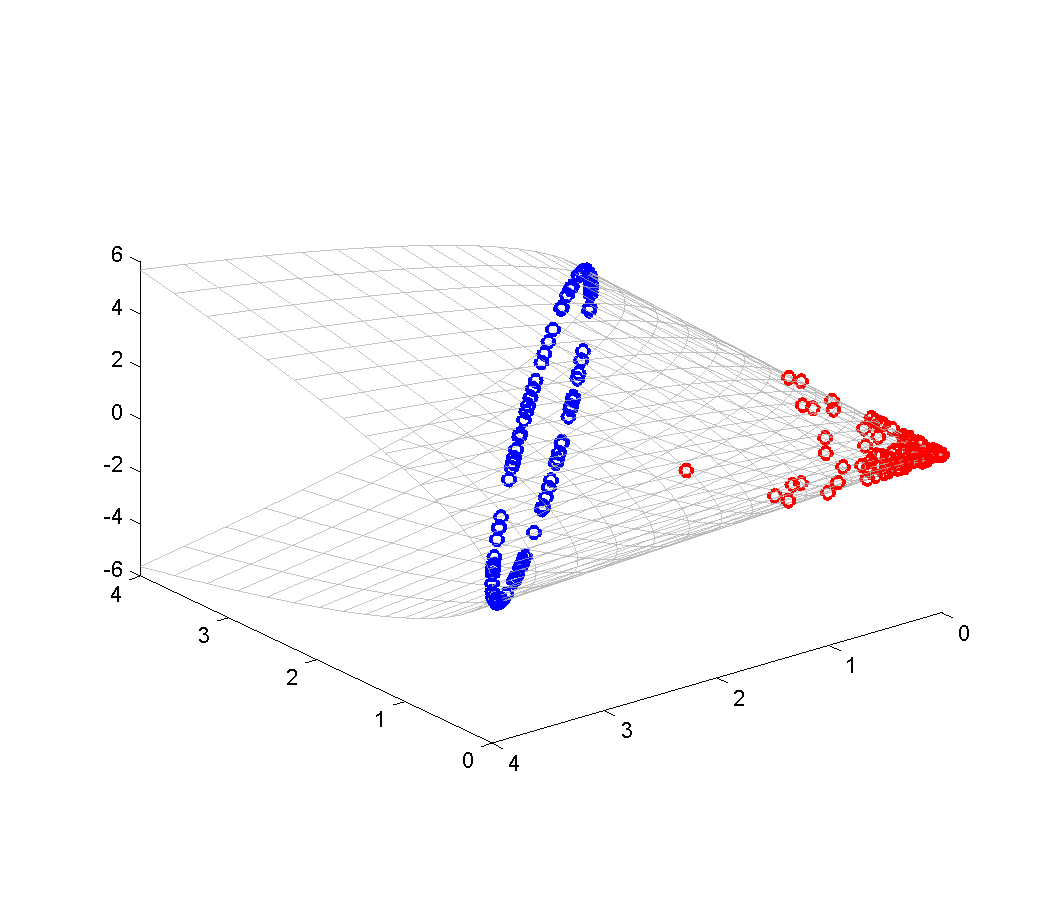
\includegraphics[width=0.45\columnwidth]{figures/fmapped_data.pdf}
    \label{fig:fmapped_data}}
     \subfloat[Linear boundary in new space.]
     {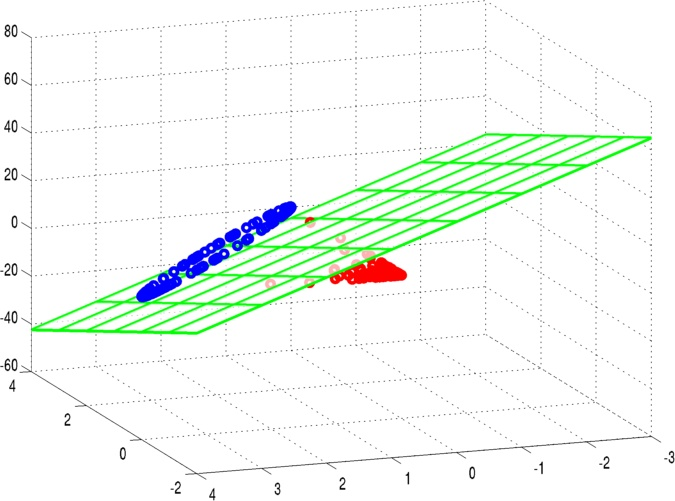
\includegraphics[width=0.45\columnwidth]{figures/pres_perc_fmapped_data_after.jpg}
     \label{fig:fmapped_bound}}  
    \caption{If we map the same data using a nonlinear map $\phi(x,y):= (x^2, y^2, 2xy)$, the perceptron now finds a solution
             in 3 dimensions.}
    \label{fig:fmapped}
    %\end{figure}
%\begin{figure}[tbh] %{r}{0.5\textwidth}
\end{figure} 